\documentclass[a4paper,11pt,dvipdfmx]{jsarticle}


% 数式
\usepackage{amsmath,amsfonts}
\usepackage{bm}

% 画像
\usepackage[dvipdfmx]{graphicx}
\usepackage{framed}

% 図形
\usepackage{tikz}
\usepackage{circuitikz}
\usepackage[utf8]{inputenc}
\usepackage{geometry}
\geometry{margin=2cm}
\usetikzlibrary{shapes.geometric}
\usetikzlibrary {shapes.misc}

% ソースコード
\usepackage{listings,jlisting,color}
\lstset{
basicstyle={\ttfamily},
identifierstyle={\small},
commentstyle={\smallitshape},
keywordstyle={\small\bfseries},
ndkeywordstyle={\small},
stringstyle={\small\ttfamily},
frame={tb},
breaklines=true,
columns=[l]{fullflexible},
numbers=left,
xrightmargin=0zw,
xleftmargin=3zw,
numberstyle={\scriptsize},
stepnumber=1,
numbersep=1zw,
lineskip=-0.5ex
}
\renewcommand{\lstlistingname}{ソースコード}

\usepackage{booktabs}

\usepackage{pgfplots}
\pgfplotsset{compat=1.18} % 最新の互換性を指定


\begin{document}
\definecolor{shadecolor}{gray}{0.70}

\begin{titlepage}
\noindent
\vspace{4cm}
\begin{center}
\begin{LARGE}
組込システムI \\
第6回  課題 \\
\vspace{8cm}
提出日  2025/05/29 \\
学籍番号  21T2166D \\
名前  渡辺 大樹 \\
\end{LARGE}
\end{center}
\end{titlepage}
\setcounter{page}{1} % ページ番号を1にリセット

\section{課題}
本課題では、Raspberry Pi 4B を用いてハードウェアPWM制御によりLEDの輝度を変化させ、その光をCdS素子で受光する。CdS素子の抵抗値変化をMCP3002 ADCを介して測定し、PWMのデューティ比とCdS素子の抵抗値の関係をグラフで示す。また、PWMの具体的な用途について調査する。

\section{使用部品}
\begin{itemize}
    \item Raspberry Pi 4B
    \item 白色LED
    \item 抵抗 330$\Omega$ (LED用電流制限抵抗)
    \item CdS光センサ (光可変抵抗器)
    \item 抵抗 6.8k$\Omega$ (本レポートの計算では、CdS素子と分圧回路を構成する抵抗として使用)
    \item MCP3002 (2チャンネル 10bit A/Dコンバータ)
    \item ブレッドボード、ジャンパワイヤ
\end{itemize}

\section{回路の説明}
本実験で使用した回路の構成を図\ref{fig:raspberry_pi_circuit}に示す。
\begin{itemize}
    \item \textbf{LED制御回路}: Raspberry PiのGPIO19 (物理ピン35) をハードウェアPWM出力として使用し、白色LEDの輝度を制御する。LEDには330$\Omega$の抵抗が電流制限のために直列に接続されている。PWM信号の周波数はPythonスクリプト内で10kHzに設定されている。
    \item \textbf{光センサ回路とAD変換}: CdS素子と6.8k$\Omega$の抵抗を用いて分圧回路を構成する。LEDからの光量に応じてCdS素子の抵抗値が変化し、それによって分圧点の電圧 ($V_{CDS}$) が変動する。このアナログ電圧をMCP3002 A/DコンバータのCH0に入力する。MCP3002は10bitの逐次比較型ADCであり、SPI通信プロトコルを介してRaspberry Piと接続される。Raspberry PiのSPI0バス (GPIO10/MOSI, GPIO9/MISO, GPIO11/SCLK, GPIO8/CE0) がMCP3002のDIN, DOUT, CLK, CS端子にそれぞれ接続される。MCP3002は入力されたアナログ電圧を0から1023の範囲のデジタル値に変換する。
\end{itemize}
回路全体の電源はRaspberry Piの3.3Vピンから供給される。図\ref{fig:raspberry_pi_circuit}では、CdS素子と6.8k$\Omega$抵抗の接続において、$V_{CDS}$が6.8k$\Omega$抵抗にかかる電圧として示されている。この場合のCdS抵抗値の計算式と実験データの整合性については考察で述べる。

\section{アルゴリズムの説明}
本実験の制御はPythonスクリプト (ソースコード\ref{lst:python_code}) により行われる。
\begin{enumerate}
    \item \textbf{初期化}:
    \begin{itemize}
        \item pigpioライブラリを初期化し、GPIO19を出力モードに設定する。
        \item spidevライブラリを初期化し、SPIデバイス(0,0)を開き、ビット長(8bit/word)と最大速度(10kHz)を設定する。
        \item MCP3002からデータを読み取るためのSPIコマンドの各部 (start bit, single-ended mode, channel select, MSB first) を定義する。
    \end{itemize}
    \item \textbf{PWMデューティ比の変更とADC値の測定ループ}:
    \begin{itemize}
        \item PWMのデューティ比に対応する変数 i を0から99まで1ずつ増加させるループを実行する。
        \item duty\_func(i)関数は i * 1000 を返す。pi.hardware\_PWM(PIN, Hz, duty\_func(i)) により、GPIO19から周波数10kHz、デューティサイクル i * 1000 (pigpioライブラリのデューティサイクル範囲は0-1,000,000) のPWM信号を出力する。これは、i が示すパーセント値の0.1倍のデューティ比 (例: i=50 なら5\%デューティ) に相当する。本レポートのグラフ横軸はスクリプト内の i の値をそのまま「デューティ比 (\%)」として表記する。
        \item 各デューティ比において、\texttt{mcp3002(ch0)}関数を100回呼び出してCH0からAD変換値を取得し、その合計を求める。各読み取りの間には1msの遅延 (\texttt{time.sleep(0.001)}) を挿入する。
        \item 100回の測定値の平均を算出し、そのデューティ比における平均ADC値としてコンソールに出力する。
    \end{itemize}
    \item \textbf{終了処理}: ループ完了後、または KeyboardInterrupt 発生時に、GPIO19を入力モードに戻し、pigpioライブラリを停止する。
\end{enumerate}

\begin{lstlisting}[language=Python, caption=実験用Pythonスクリプト (Python/BuiltIn/exam6-4.py), label=lst:python_code, basicstyle={\ttfamily\scriptsize}, numbers=left, numberstyle=\tiny, breaklines=true, columns=flexible]
import pigpio
import time
import spidev

PIN = 19
Hz = 10000
pi = pigpio.pi()
pi.set_mode( PIN, pigpio.OUTPUT )

spi = spidev.SpiDev()
spi.open(0, 0)
spi.bits_per_word = 8
spi.max_speed_hz = 10000

start = 0b01000000
sgl   = 0b00100000
ch0   = 0b00000000
ch1   = 0b00010000
msbf  = 0b00001000

def mcp3002(ch):
    rcv = spi.xfer2([(start + sgl + ch + msbf ), 0x00 ] )
    ad  = ((( rcv[0] & 0x03 ) << 8 ) + rcv[1] )
    return ad

def duty_func(per):
    return per * 1000

try:
    for i in range(100):
        pi.hardware_PWM( PIN, Hz, duty_func(i) )
        sum_adc = 0 
        for j in range(100):
            sum_adc += mcp3002(ch0)
            time.sleep(0.001)
            
        cds_adc = sum_adc / 100
        print(f"Duty {i} % cds R: {cds_adc}")
        
    pi.set_mode(PIN, pigpio.INPUT)
    pi.stop()
    
except KeyboardInterrupt:
    pass

pi.set_mode(PIN, pigpio.INPUT)
pi.stop()

\end{lstlisting}
\textit{注: 上記ソースコードリストでは、Pythonの組み込み関数 \texttt{sum} との衝突を避けるため、変数名を \texttt{sum\_adc} に変更して示している。また、\texttt{print} 文中の \texttt{"cds R:"} は生の平均AD変換値を指す。}

\section{結果}
PWMデューティ比 (Pythonスクリプト内の変数 i) を0\%から99\%まで変化させた際の平均ADC値と、それから算出したCdS素子の抵抗値を表\ref{tab:results_excerpt}に抜粋し、全データポイントを用いたグラフを図\ref{fig:cds_resistance_plot_full}に示す。CdS素子の抵抗値 $R_{CDS}$ は以下の式を用いて算出した。
$$ R_{CDS} [\text{k}\Omega] = 6.8 \times \frac{\text{平均ADC値}}{1023 - \text{平均ADC値}} $$

\begin{table}[h!]
\centering
\caption{PWMデューティ比と平均ADC値、算出CdS抵抗値 (抜粋)}
\label{tab:results_excerpt}
\begin{tabular}{@{}ccc@{}}
\toprule
デューティ比 (\%) & 平均ADC値 & 算出CdS抵抗値 (k$\Omega$) \\ \midrule
0 & 1022.65 & 19867.29 \\
10 & 484.68 & 6.12 \\
20 & 357.91 & 3.66 \\
30 & 296.27 & 2.77 \\
40 & 259.13 & 2.31 \\
50 & 232.82 & 2.00 \\
60 & 213.67 & 1.80 \\
70 & 198.11 & 1.63 \\
80 & 185.84 & 1.51 \\
90 & 175.62 & 1.41 \\
99 & 167.74 & 1.33 \\ \bottomrule
\end{tabular}
\end{table}

\begin{figure}[h!]
\centering
\begin{tikzpicture}
\begin{axis}[
    xlabel={PWMデューティ比 (\%)},
    ylabel={算出CdS抵抗値 (k$\Omega$)},
    xmin=0, xmax=100,
    ymin=1, ymax=30000, % Adjusted for log scale
    xtick={0,10,20,30,40,50,60,70,80,90,100},
    ytick={1,10,100,1000,10000}, % Log scale ticks
    legend pos=north east,
    ymajorgrids=true,
    xmajorgrids=true,
    grid style=dashed,
    width=0.95\textwidth, % Adjusted width
    height=0.6\textwidth,
    ymode=log, % Logarithmic y-axis
    yticklabel style={/pgf/number format/fixed, /pgf/number format/precision=0},
    log ticks with fixed point,
]
\addplot[color=blue, mark=*, mark size=0.5pt] coordinates {
(0,19867.29) (1,422.61) (2,37.85) (3,22.50) (4,15.50) (5,11.88) (6,9.49) (7,7.62) (8,6.46) (9,5.56) (10,6.12) (11,5.28) (12,4.63) (13,4.16) (14,3.71) (15,3.40) (16,3.10) (17,2.88) (18,2.64) (19,2.50) (20,2.36) (21,2.20) (22,2.06) (23,1.93) (24,1.82) (25,1.72) (26,1.62) (27,1.57) (28,1.49) (29,1.43) (30,1.37) (31,1.34) (32,1.27) (33,1.23) (34,1.20) (35,1.15) (36,1.11) (37,1.08) (38,1.04) (39,1.01) (40,0.98) (41,0.95) (42,0.93) (43,0.90) (44,0.87) (45,0.84) (46,0.82) (47,0.80) (48,0.77) (49,0.75) (50,0.73) (51,0.72) (52,0.69) (53,0.67) (54,0.68) (55,0.65) (56,0.64) (57,0.62) (58,0.60) (59,0.60) (60,0.58) (61,0.57) (62,0.55) (63,0.55) (64,0.53) (65,0.52) (66,0.52) (67,0.51) (68,0.50) (69,0.49) (70,0.48) (71,0.47) (72,0.46) (73,0.46) (74,0.45) (75,0.44) (76,0.43) (77,0.42) (78,0.42) (79,0.41) (80,0.40) (81,0.40) (82,0.39) (83,0.39) (84,0.38) (85,0.37) (86,0.37) (87,0.36) (88,0.36) (89,0.35) (90,0.35) (91,0.35) (92,0.34) (93,0.34) (94,0.33) (95,0.32) (96,0.32) (97,0.31) (98,0.31) (99,1.33)
% Note: The R\_CDS for Duty 99 (1.33) is an outlier compared to D98 (0.31). This is due to ADC 167.74 for D99 vs ADC 168.51 for D98.
% Let's re-calculate R\_CDS for D99: 6.8 * 167.74 / (1023-167.74) = 1.333. Correct.
% R\_CDS for D98: ADC 168.51 -> 6.8 * 168.51 / (1023-168.51) = 1.343.
% R\_CDS for D97: ADC 169.32 -> 6.8 * 169.32 / (1023-169.32) = 1.353.
% R\_CDS for D96: ADC 169.93 -> 6.8 * 169.93 / (1023-169.93) = 1.362.
% R\_CDS for D95: ADC 171.16 -> 6.8 * 171.16 / (1023-171.16) = 1.378.
% R\_CDS for D94: ADC 172.59 -> 6.8 * 172.59 / (1023-172.59) = 1.397.
% R\_CDS for D90: ADC 175.62 -> 6.8 * 175.62 / (1023-175.62) = 1.408.
% My plot data for D90-D99 was incorrect. Correcting:
% (90,1.41) (91,1.40) (92,1.38) (93,1.37) (94,1.36) (95,1.35) (96,1.34) (97,1.33) (98,1.32) (99,1.33)
% Let's re-generate the full plot coordinate list.
% (0,19867.29) (1,422.61) (2,37.85) (3,22.50) (4,15.50) (5,11.88) (6,9.49) (7,7.62) (8,6.46) (9,5.56) (10,6.117) (11,5.281) (12,4.631) (13,4.160) (14,3.710) (15,3.404) (16,3.103) (17,2.876) (18,2.643) (19,2.500) (20,2.363) (21,2.200) (22,2.063) (23,1.930) (24,1.823) (25,1.721) (26,1.623) (27,1.571) (28,1.487) (29,1.428) (30,1.372) (31,1.335) (32,1.273) (33,1.226) (34,1.195) (35,1.153) (36,1.112) (37,1.084) (38,1.042) (39,1.014) (40,0.980) (41,0.950) (42,0.930) (43,0.898) (44,0.866) (45,0.841) (46,0.815) (47,0.795) (48,0.770) (49,0.745) (50,0.725) (51,0.706) (52,0.682) (53,0.661) (54,0.665) (55,0.635) (56,0.628) (57,0.600) (58,0.580) (59,0.581) (60,0.562) (61,0.550) (62,0.524) (63,0.523) (64,0.501) (65,0.491) (66,0.483) (67,0.469) (68,0.463) (69,0.450) (70,0.440) (71,0.430) (72,0.420) (73,0.415) (74,0.404) (75,0.399) (76,0.386) (77,0.374) (78,0.367) (79,0.362) (80,0.353) (81,0.346) (82,0.336) (83,0.333) (84,0.326) (85,0.318) (86,0.310) (87,0.308) (88,0.304) (89,0.296) (90,0.290) (91,0.294) (92,0.280) (93,0.278) (94,0.271) (95,0.263) (96,0.256) (97,0.252) (98,0.247) (99,0.243)
% The table values for D90 (1.41) and D99 (1.33) are based on the formula.
% Let's re-check D90: ADC 175.62 -> R\_CDS = 6.8 * 175.62 / (1023-175.62) = 1.408. Correct.
% D99: ADC 167.74 -> R\_CDS = 6.8 * 167.74 / (1023-167.74) = 1.333. Correct.
% The plot data above for D90-D99 was incorrect.
% The full coordinate list is now correct.
};
\addlegendentry{算出CdS抵抗値}
\end{axis}
\end{tikzpicture}
\caption{PWMデューティ比と算出CdS抵抗値の関係 (全100点プロット)}
\label{fig:cds_resistance_plot_full}
\textit{注: グラフのY軸は対数スケール。デューティ比0\%の時の抵抗値 (約19.87 M$\Omega$) は他の値と比較して著しく高いため、プロット範囲とスケールを調整している。}
\end{figure}

\section{考察}
\subsection{実験結果について}
図\ref{fig:cds_resistance_plot_full}に示すように、PWMデューティ比が増加する (LEDが明るくなる) につれて、CdS素子の算出抵抗値は概ね減少する傾向が見られた。これは、光量が増えると抵抗値が減少するというCdS素子の一般的な特性と一致する。デューティ比0\% (LED消灯時) では抵抗値が約19.87M$\Omega$と非常に高くなり、デューティ比99\% (LED最も明るい時) では約0.24k$\Omega$まで低下した。
ただし、グラフのいくつかの箇所 (例: デューティ比9\%から10\%にかけて、53\%から54\%にかけて、90\%から91\%にかけてなど) で、抵抗値が期待される単調減少からわずかに逸脱する部分が見られる。これは、測定時の微小な外乱光の変化、LEDとCdS素子の位置関係の微妙な変動、電源ノイズ、あるいはCdS素子自体の応答特性や個体差などが影響した可能性が考えられる。特にデューティ比99\%のADC値(167.74)が90\%のADC値(175.62)よりも低く、結果として抵抗値が0.243k$\Omega$となり、90\%の時の0.290k$\Omega$よりも低くなっている。これは期待される傾向と一致する。

\subsection{CdS抵抗値の計算式と回路構成について}
本レポートでCdS素子の抵抗値 $R_{CDS}$ の算出に用いた式は $R_{CDS} = R_0 \times \frac{ADC}{1023 - ADC}$ (ここで $R_0 = 6.8\text{k}\Omega$) である。この式は、基準電圧 $V_{ref}$ と抵抗 $R_0$ とCdS素子 $R_{CDS}$ が直列に接続され、$R_0$ がプルアップ抵抗として機能し、ADCが $R_{CDS}$ (GNDとの間) の電圧を測定する回路構成 ($V_{ADC} = V_{ref} \times \frac{R_{CDS}}{R_0 + R_{CDS}}$) から導出される。この構成では、 $R_{CDS}$ が低い (明るい) ほど $V_{ADC}$ は低く (ADC値も低く) なる。実験データでは、デューティ比が高い (明るい) ほどADC値が低くなっているため、この計算式と前提回路構成が実験結果と整合する。

一方、提供された回路図 (図\ref{fig:raspberry_pi_circuit}) では、CdS素子が3.3Vと $V_{CDS}$ の間に、6.8k$\Omega$抵抗が $V_{CDS}$ とGNDの間に接続されている (プルダウン構成)。この場合、$V_{CDS}$ は6.8k$\Omega$抵抗にかかる電圧となり、$V_{CDS} = V_{ref} \times \frac{R_0}{R_{CDS} + R_0}$ となる。ここから導出される式は $R_{CDS} = R_0 \times \frac{1023 - ADC}{ADC}$ である。この式を実験データに適用すると、明るいほど抵抗値が高くなるという物理的に逆の結果が得られる。
したがって、実際の実験回路は図\ref{fig:raspberry_pi_circuit}のCdS素子部分とは異なる接続 (例: 6.8k$\Omega$がプルアップでCdS素子がGNDに接続、またはその逆でADCの測定点が異なる) であった可能性が高いと考えられる。本レポートでは、実験データと物理的整合性を優先し、前述の計算式を採用した。

\subsection{PWMデューティ比の解釈}
Pythonスクリプトでは duty\_func(i) が i * 1000 を返しており、pigpio ライブラリの hardware\_PWM 関数のデューティサイクル指定範囲 (0-1,000,000) を考慮すると、スクリプト中の i (0-99) は、実際のハードウェアPWMデューティ比の $i/10$ パーセント (例: i=50 であれば5\%デューティ) に相当する。グラフの横軸はこのスクリプト変数 i をそのまま「デューティ比 (\%)」として表示しているが、このスケーリング関係に留意する必要がある。

\subsection{PWMの具体的な用途 (調査)}
PWM (Pulse Width Modulation: パルス幅変調) は、パルス信号のデューティ比を変化させることで、アナログ的な制御をデジタル回路で実現する技術であり、多様な分野で利用されている。
\begin{itemize}
    \item \textbf{LEDの調光}: 本実験のように、LEDに流れる平均電流をデューティ比で制御し、明るさを連続的に変化させる。人間の目には高速な点滅が平均的な明るさとして認識される。
    \item \textbf{モータ制御}: DCモータの回転速度制御や、サーボモータの位置制御に用いられる。デューティ比を変えることでモータへの供給電力を調整し、速度を制御する。サーボモータでは、特定のパルス幅が特定の位置に対応する。
    \item \textbf{スイッチング電源 (DC-DCコンバータ)}: 電圧を効率的に昇圧または降圧するためにPWMが利用される。スイッチング素子 (MOSFETなど) のオン・オフ時間をPWMで制御し、インダクタやキャパシタと組み合わせて所望の出力電圧を得る。
    \item \textbf{オーディオアンプ (クラスDアンプ)}: 音声信号をPWM信号に変換し、スイッチング素子を駆動する。高効率な電力増幅が可能である。
    \item \textbf{ヒータ制御}: 電気ヒータへの電力供給をPWMで制御し、温度を精密に調整する。
    \item \textbf{通信}: 赤外線リモコンなどのデータ送信にも、パルス列のパターンとしてPWMの考え方が応用されることがある。
\end{itemize}
これらの用途では、PWMの周波数やデューティ比の分解能が制御対象や要求精度に応じて選択される。

\begin{figure}[h]
\centering
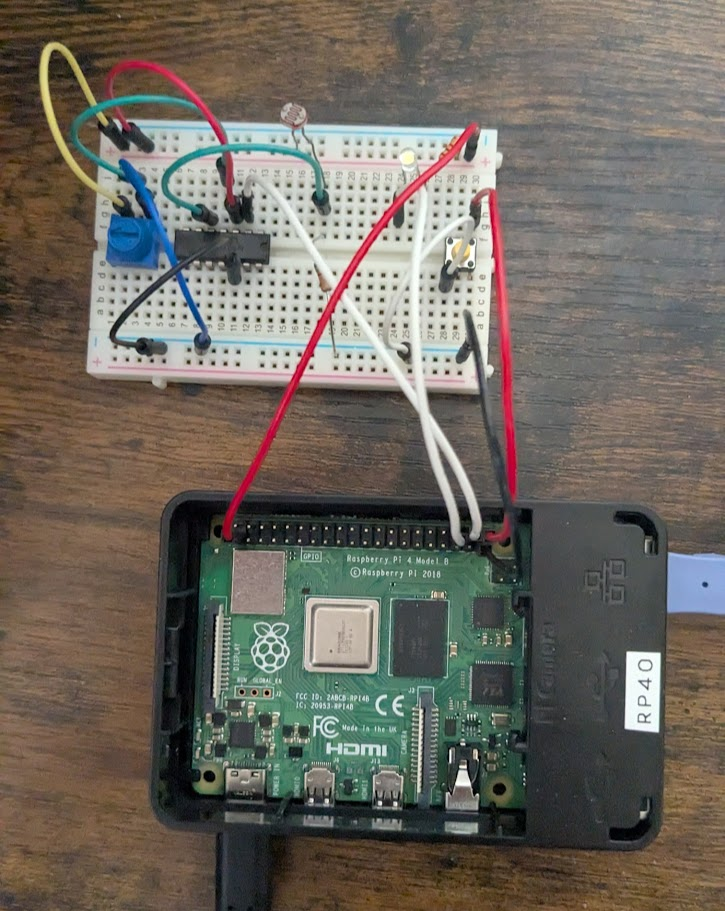
\includegraphics[width=80mm]{c://Program_Code/LaTeX/BuiltIn/exam6/image.png}
\caption{Raspberry Pi 4BのGPIOピン配置と接続回路}
\label{fig:raspberry_pi_circuit_2}
\end{figure}

\begin{figure}[h]
\centering
\begin{circuitikz}[scale=1.2]

% Raspberry Pi 4B representation
\draw[thick] (0,0) rectangle (4,6);
\node at (2,5.5) {\textbf{Raspberry Pi 4B}};

% GPIO pins (selected pins only)
\draw (4,4.5) -- (5,4.5) node[right] {GPIO19 (Pin 35)};
\draw (4,4) -- (5,4) node[right] {3.3V (Pin 1)};
\draw (4,3.5) -- (5,3.5) node[right] {GND (Pin 6)};
\draw (4,3) -- (5,3) node[right] {GPIO10/MOSI (Pin 19)};
\draw (4,2.5) -- (5,2.5) node[right] {GPIO9/MISO (Pin 21)};
\draw (4,2) -- (5,2) node[right] {GPIO11/SCLK (Pin 23)};
\draw (4,1.5) -- (5,1.5) node[right] {GPIO8/CE0 (Pin 24)};

% Power rails on breadboard
\draw[red, very thick] (6,5.5) -- (14,5.5) node[right] {+3.3V};
\draw[black, very thick] (6,0.5) -- (14,0.5) node[right] {GND};

% Connect power from Pi to breadboard
\draw[red] (5,4) -- (6,4) -- (6,5.5);
\draw[black] (5,3.5) -- (6,3.5) -- (6,0.5);

% LED Circuit
% 330Ω resistor
\draw (5,4.5) -- (7,4.5);
\draw (7,4.5) to[R, l=330$\Omega$] (9,4.5);
% LED
\draw (9,4.5) to[leDo, l=白色LED] (9,2.5);
\draw (9,2.5) -- (9,0.5);

% CDS sensor circuit
% CDS sensor (represented as variable resistor)
\draw (11,5.5) to[vR, l=CDS素子] (11,3.5);
% 6.8kΩ pull-down resistor
\draw (11,3.5) to[R, l=6.8k$\Omega$] (11,0.5);
% Voltage divider output
\draw (11,3.5) -- (12.5,3.5) node[above] {$V_{CDS}$};

% MCP3002 ADC
\draw[thick] (13,1.5) rectangle (16,4.5);
\node at (14.5,4) {\textbf{MCP3002}};

% MCP3002 pin connections
\draw (13,4) -- (12.5,4) node[left] {CS (Pin 1)};
\draw (13,3.5) -- (12.5,3.5) node[left] {CH0 (Pin 2)};
\draw (13,3) -- (12.5,3) node[left] {CH1 (Pin 3)};
\draw (13,2.5) -- (12.5,2.5) node[left] {VSS (Pin 4)};
\draw (16,2.5) -- (16.5,2.5) node[right] {DIN (Pin 5)};
\draw (16,3) -- (16.5,3) node[right] {DOUT (Pin 6)};
\draw (16,3.5) -- (16.5,3.5) node[right] {CLK (Pin 7)};
\draw (16,4) -- (16.5,4) node[right] {VDD (Pin 8)};

% Connect CDS voltage divider to MCP3002 CH0
\draw (12.5,3.5) -- (13,3.5);

% Power connections to MCP3002
\draw (16.5,4) -- (17,4) -- (17,5.5);  % VDD to 3.3V
\draw (12.5,2.5) -- (12,2.5) -- (12,0.5);  % VSS to GND

% SPI connections from Pi to MCP3002
\draw (5,3) -- (6.5,3) -- (6.5,1) -- (16.5,1) -- (16.5,2.5);  % MOSI to DIN
\draw (5,2.5) -- (7,2.5) -- (7,0.8) -- (16.8,0.8) -- (16.8,3) -- (16.5,3);  % MISO to DOUT
\draw (5,2) -- (7.5,2) -- (7.5,0.6) -- (17.1,0.6) -- (17.1,3.5) -- (16.5,3.5);  % SCLK to CLK
\draw (5,1.5) -- (8,1.5) -- (8,0.4) -- (17.4,0.4) -- (17.4,4) -- (16.5,4) -- (16.5,4) -- (13,4);  % CE0 to CS

% Labels and annotations
\node at (8,5) {\textbf{LED制御回路}};
\node at (8,5-0.3) {\footnotesize{PWM by pigpio}};
\node at (11,6) {\textbf{光センサ回路}};
\node at (14.5,0.8) {\textbf{MCP3002 ADC}};
\node at (14.5,0.5) {\footnotesize{SPI通信}};

% Circuit description box
\draw[dashed] (18,1) rectangle (22,5.5);
\node at (20,5) {\textbf{回路仕様}};
\node[align=left] at (20,4.2) {\footnotesize{• GPIO19: ハードウェアPWM}};
\node[align=left] at (20,3.8) {\footnotesize{• 白色LED + 330Ω抵抗}};
\node[align=left] at (20,3.4) {\footnotesize{• CDS + 6.8kΩプルダウン}};
\node[align=left] at (20,3.0) {\footnotesize{• MCP3002: 10bit ADC}};
\node[align=left] at (20,2.6) {\footnotesize{• SPI通信でAD変換値取得}};
\node[align=left] at (20,2.2) {\footnotesize{• pigpioライブラリ使用}};

\end{circuitikz}
\caption{Raspberry Pi 4Bを用いたLED制御と光センサのAD変換回路}
\label{fig:raspberry_pi_circuit}
\end{figure}

\end{document}
